\section{Implementation} \label{sec:implementation}

We now discuss implementation details for the major system components discussed in Section~\ref{sec:grappa}.

\subsection{Memory}

Grappa implements a software distributed shared memory. This memory is exposed
through two distinct, non-overlapping address spaces; one optimized for global
access to node-local data, and another optimized for high aggregate random
access bandwidth to low locality data.

All global addresses in Grappa are 64-bit
values. Each byte of global memory is associated with a {\em home core}; this
core is responsible for allocating and modifying that memory. Since today's
commodity processors support a 48-bit virtual address space \TODO{cite?},
Grappa uses the spare bits to distinguish which address space a global address
belongs to, and to represent the home core of a global address.

\begin{figure}[t]
\begin{center}
  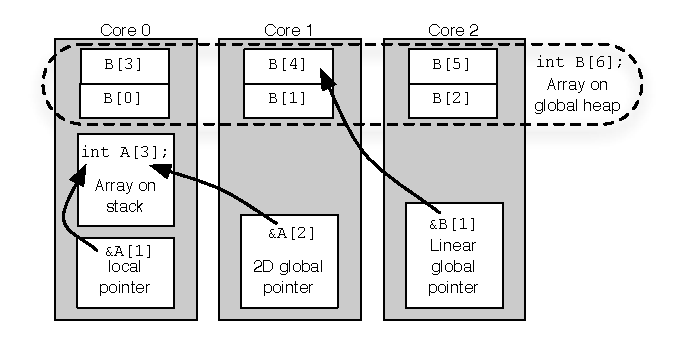
\includegraphics[width=0.95\columnwidth]{figs/memory-structure}
\begin{minipage}{0.95\columnwidth}
  \caption{\label{fig:memory-structure} Grappa memory structure}
\end{minipage}
\vspace{-3ex}
\end{center}
\end{figure}


\paragraph{2D global addresses} The first global address space is the {\em
two-dimensional} address space. This uses a traditional PGAS addressing model,
where each address is a tuple of a rank in the job (or global process ID) and
an address in that process. The lower 48 bits of the address hold a virtual
address in the process. The top bit is set to indicates that the reference is
a 2D address. This leaves 15 bits for network endpoint ID, which limits our
scalability to $2^{15}$ endpoints.

Any node-local data can be made accessible by other nodes in the system by
wrapping the address and node ID into a 2D global address. This address can
then be accessed with delegate and can also be cached by other nodes. At the
destination the address is converted into a canonical x86 address by replacing
the upper bits with the sign-extended upper bit of the virtual address.

\paragraph{Linear global addresses} The second global address space is the {\em linear} address space, so
named because nearby addresses can be treated as adjacent even if they
are stored on different nodes. Addresses in the linear address space
are partitioned across the cluster in a block-cyclic fashion. Choosing
the block size involves trading off sequential bandwidth against
aggregate random access bandwidth. Smaller block sizes help spread
data across all the memory controllers in the cluster, but larger
block sizes allow the locality-optimized memory controllers to provide
increased sequential bandwidth. The block size, which is configurable, is typically set to 64
bytes, or the size of a single hardware cache line, in order to
exploit spatial locality when available. 

All linear addresses refer to data allocated from a global heap. The
heap metadata is stored on a single node. Currently all heap
operations serialize through this node; while this has been sufficient
for our benchmarks, parallel performance can be achieved through
combining \TODO{ cite MAMA and flat combining}. 2D addresses may refer
to memory allocated from a single processes' heap or from a task's
stack. Figure~\ref{fig:memory-structure} shows how 2D and linear
addresses can refer to other cores' memory.

\TODO{Add a figure that depicts both forms of global addresses.}

All global memory operations are implemented with active
messages. Requesters construct a descriptor holding the current task
ID and space for a response, issue their request active message to the
node given by the request address, and suspend themselves. When the
request arrives at the address' home node, the operation is performed
and a response active message is sent. When the response arrives at
the requesting node, the descriptor is filled in with the results of
the operation and the requesting task is woken.

\paragraph{Delegates} Delegate operations are used for low-locality accesses and synchronization. Their modifications
are always executed at the home core of their address, and while
arbitrary memory operations can be delegated, we restrict the use of
delegate operations in three ways to make them more useful for
synchronization. First, we limit each task to one outstanding delegate
operation to avoid the possibility of reordering in the
network. Second, we limit delegate operations to operate on objects in
the 2D address space or objects that fit in a single block of the
linear address space so they can be satisfied with a single network
request. Finally, no context switches are allowed while the data is
being modified. Given these restrictions, we can ensure that delegate
operations for the same address from multiple requesters are always
serialized through a single core in the system, providing atomic
semantics without using atomic operations.

\paragraph{Explicit caches} Grappa cache operations are used to exploit
spatial or temporal locality. They allow a single task to buffer a range of
data, read or modify it, and write the modified version back to its home node.
All fetch and update operations of cache data are expressed explicitly by the
programmer. Cache operations may operate on data that spans multiple blocks of
the linear address space; the programmer provides the starting address and
length, and the cache issues as many active messages as necessary to retrieve
all necessary data.

\comment{If anything, this is just a footnote. -M
All current cache operations are incoherent; two tasks may
concurrently modify the same block with their writes interfering
unless protected by synchronization through delegate operations. While
this has been sufficient for our benchmarks, it is possible to embed
synchronization in the cache active messages and reduce the number of
network round trips necessary.}


\subsection{Tasking}

\subsubsection{Tasks and workers}

Grappa tasks are 32-byte entities: a 64-bit function pointer plus
three 64-bit arguments. We use three arguments because tasks are
usually generated as part of a parallel loop decomposition, and thus
each task needs three kinds of data.
\begin{description}
\item[Function pointer] This 64-bit value indicates what routine
  should run. We configure the system nodes to disable address randomization, so that we can depend on the fact that function pointers are valid across process images.
\item[Private argument] This 64-bit value is typically used for task-specific
  data (e.g., a loop index).
\item[Shared argument] This 64-bit value is typically used for data shared
  between all tasks that are part of a loop or to specify the number
  of loop iterations.
\item[Synchronization argument] This 64-bit value is typically used to determine
  when all tasks that are part of a loop have finished. It is usually
  a global pointer to a synchronization object allocated at the core
  that spawned the task.
\end{description}
While these are the most common uses of the three task arguments, they
are treated as arbitrary 64-bit values in the runtime, and can be used
for any purpose.

Tasks are not allocated any execution resources until the scheduler
decides to run them; when this occurs, tasks are matched with {\em
  worker} threads. Each worker is simply a collection of status bits and a
stack, allocated at a particular core.


\subsubsection{Context switching}

Context switching in Grappa is non-preemptive. Any Grappa routine that
does a potentially-long-latency operation calls a context-switch
routine that gives control of the core back to the scheduler. Users
may also explicit yield control to the scheduler.

As with other cooperative multithreading systems, we treat context
switches as function calls, saving and restoring only the callee-saved
state as specified in the x86-64 ABI \TODO{cite}. This involves saving
six general-purpose 64-bit registers and the stack pointer, as well as
the 16-bit x87 floating point control word and the SSE context/status
register. Thus, the minimum amount of state a cooperative context
switch routine must save according to the ABI is 62 bytes.

Since the compiler sees all calls to the context switch routine, we
can save even less state. Our context switch routine appears to the
compiler as inline assembly; we declare all the registers we need
to save as ``clobbered'' by the inline assembly routine, and the
compiler will issue its own save and restore code as needed. This allows the
compiler to avoid saving any registers that are not used, or are used
for temporary values that are not needed after the context switch.
\comment{I highly doubt this is important in real apps beyond our kernels.  -M
Why not? liveness is a common compiler analysis -BM

In
particular, only one of our applications does floating point
operations; all the other applications can safely ignore the x87 and
SSE2 registers as part of context switching.}

\subsubsection{Scheduling}

Each core in the Grappa system has its own independent scheduler. Each
scheduler has three main tasks to perform.  First, it must ensure that
its communication resources are serviced reasonably often. Second, it
must ensure that if a running task was waiting on a long-latency
operation and that operation has completed, the task will be
rescheduled. Third, if there are tasks waiting to be run and spare
execution resources, the tasks must be matched with idle workers.

Each scheduler has three queues:
\begin{description}
\item{\bf Ready worker queue} This is a FIFO queue of tasks that are
  matched with workers and are ready to execute.
\item{\bf Private task queue} This is a FIFO queue of tasks that must run on this core.
\item{\bf Public task queue} This is a LIFO queue of tasks that are
  waiting to be matched with workers. It is a local partition of a shared
  task pool; this is described in the next section.
\end{description}

Whenever a task yields or suspends, the scheduler makes a decision
about what to do next. First, it determines if
the communication resources should be serviced. This is done on a
periodic basis. Second, it determines if any workers with running
tasks are ready to execute; if so, one is scheduled. Finally, if there
are no workers ready to run, but there are tasks waiting to be matched
with workers, an idle worker is woken (or a new worker is spawned),
matched with a task, and scheduled.

The scheduler uses its core's timestamp counter to track time. The
timestamp counter is read once per scheduling decision. Timestamp
values are not shared between cores. We use timestamp values only to
ensure periodic execution of communication maintenance tasks; being
wrong will only change the rate of these events with a potential
performance cost, but does not cause a correctness violation. Nevertheless, we
assume Grappa will run on machines with modern timestamp counter
implementations that are monotonic and frequency-compensated.

\subsubsection{Work stealing} \label{subsec:implementation-worksteal}
When a \checkme{grappa-process} runs
out of work, it becomes a ``thief'' and asks another other
\checkme{grappa-process} (``victim'') for work. If the victim has tasks
to spare in its public queue, they will be transferred to the thief's public queue.

Most study of work stealing assumes that a processor has one worker
thread and so it only steals when utilization would go to zero. 
Grappa, on the other hand, relies on having many worker threads per core. The
core would be fully-utilized if there is always something on the ready
queue. Even if there are many active tasks, if they are all suspended
for long-latency network requests, then the core is underutilized.
So, there is a choice: should the core use some of this idle time to
perform work stealing or should it just wait as it is possible that local tasks will
create more work. We choose to have a core initiate a steal when all
of the following conditions hold: no workers are ready to run, 
the unstarted task queues are empty, and there are no outstanding steal requests. 
Having only one outstanding steal request throttles steals to
prevent flooding the network, but other scalable quieting mechanisms
would be possible, such as a voting tree\cite{scalableWorkStealingOrCilk98}
or lifelines \cite{lifelines}. Termination detection is not
built into the Grappa task scheduler, rather, it is considered a programming error for
the program to exit without syncing all tasks.

\TODO{where to put the following related}
Fork join computations: implement with futures or continuation passing
style
feed-forward computations: implement with scalable task counting (we
focus on this style in our benchmarks)
(briefly describe global task joiner)

choices we've made
-random victims
-steal from FIFO side of queue
-steal when at the moment readyQ empty and task queues empty
-steal min(chunk\_size, half)

Recent work has explored scalable work stealing in terms of efficient
termination detection. 



\subsection{Communication}

In order to mitigate the low message injection rate limits of commodity
networks, Grappa's communication stack has two layers: one for
user-level messages and one for network-level messages. 

At the upper layer, Grappa implements asynchronous active messages
\TODO{cite vonEicken92}. Each message consists of a function pointer, an
optional argument payload, and an optional data payload. When a task
sends a message, the message is copied to a send queue associated with
the message's destination and the task continues execution.

Grappa's lower networking layer aggregates the upper layer's messages
to improve performance. Commodity networks including Infiniband
achieves their peak injection bandwidth \emph{only} when the packet
sizes are relatively large---on the order of multiple kilobytes. The
reason for this discrepancy is the combination of overheads associated
with handling each packet (in terms of bytes that form the actual
Infiniband packet, processing time at the card and processing on the
CPU within the driver stack). Our measurements confirm manufacturers
published data~\cite{infinibandbandwidth}, that with this packet size
the bisection bandwidth is only a small fraction, less than
~\checkme{5\%} of the peak bisection bandwidth.

In our experiments the vast majority of requests were smaller than
\checkme{255}
bytes \TODO{more precise? median?}, far too small to make efficient
use of the network. To make the best use of the network, we must
convert our small messages into large ones.
\TODO{reference to aggregation evaluation later in the paper}

Grappa leverages its lightweight context switching to do this
conversion. When a task sends a message, the message is not
immediately sent. Instead, it is stored in a queue associated with its
destination, to be sent later. If the task requires a response, it
suspends itself and the scheduler finds other work to run while the
task is waiting. When the reply arrives, the suspended task is woken.

There are three situations in which a queue of aggregated messages is
sent. First, each queue has a message size threshold, chosen to give
reasonable network performance. If the size in bytes of a queue is
above the threshold, the contents of the queue are sent
immediately. Second, each queue has a wait time threshold. If the
oldest message in a queue has been waiting longer than this threshold,
the contents of the queue are sent immediately, even if the queue size
is lower than the message size threshold.  Third, queues may be
explicitly flushed in situations where the programmer wants to
minimize the latency of a message at the cost of bandwidth
utilization.

The network layer is serviced by polling. Periodically when a context
switch occurs, the Grappa scheduler switches to the network polling
thread. This thread has three responsibilities. First, it polls the
lower-level network layer to ensure it makes progress. Second, it
deaggregates received messages and executes active message
handlers. Third, it checks to see if any aggregation queues have
messages that have been waiting longer than the threshold; if so, it
sends them.

Underneath the aggregation layer, Grappa uses the \gasnet~communication
library \TODO{cite GASNet} to actually move data. All interprocess
communication, whether on or off a cluster node, is handled by the
\gasnet~library. \gasnet~is able to take advantage of many communication
mechanisms, including Ethernet and Infiniband between nodes, as well as
shared memory within a node.

Some networks provide access to a remote machine's memory
directly. This would seem to be a good fit for a programming model
focused on global shared memory, but in fact we do not use it. RDMA
operations are subject to the same message rate limitations as all
other messages on these cards, and thus using raw RDMA operations for
our small messages would make inefficient use of bandwidth. Instead,
we implement remote memory operations with active messages. A byproduct of this design decision is that Grappa is not limited
to RDMA-capable networks.
